\documentclass{article}
\usepackage{tikz}
\usetikzlibrary{calc,trees,positioning,arrows,chains,shapes.geometric,%
    decorations.pathreplacing,decorations.pathmorphing,shapes,%
    matrix,shapes.symbols}

\tikzset{
>=stealth',
  graphnode/.style={
    rectangle, 
    rounded corners, 
    % fill=black!10,
    draw=black, very thick,
    text width=10em, 
    minimum height=3em, 
    text centered, 
    on chain},
  line/.style={draw, thick, <-},
  element/.style={
    tape,
    top color=white,
    bottom color=blue!50!black!60!,
    minimum width=8em,
    draw=blue!40!black!90, very thick,
    text width=10em, 
    minimum height=3.5em,  
    text centered, 
    on chain},
  every join/.style={->, thick,shorten >=1pt},
  decoration={brace},
  hsplit/.style={decorate}
}
\begin{document}
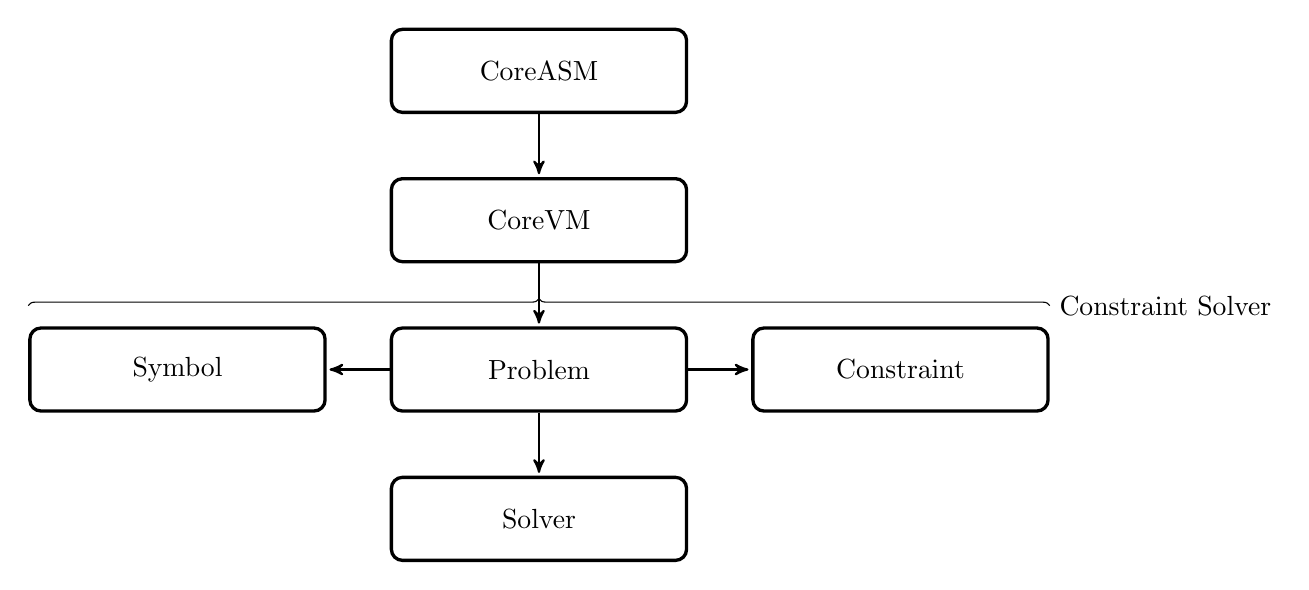
\begin{tikzpicture}
  [node distance=.8cm,
  start chain=going below,]
  
  \node[graphnode, join] {CoreASM}; 
  \node[graphnode, join] {CoreVM};

  \node[graphnode, join] (Problem) {Problem};
  \begin{scope}[start branch=venstre]
        \node[graphnode, on chain=going left, join] (Symbol) {Symbol};
  \end{scope}
  \begin{scope}[start branch=venstre]        
  	\node[graphnode, on chain=going right, join] (Constraint) {Constraint};
  \end{scope}

  \node[graphnode, join] (Solver) {Solver};

  \draw[hsplit] let
    \p1=(Symbol.west), \p2=(Constraint.east), \p3=(Problem.north) in
    ($(\x1,\y3+.75em)$) -- ($(\x2,\y3+.75em)$) node[above, right]  {Constraint Solver};
  \end{tikzpicture}
\end{document}
